%% \textbf{Project Narrative} %(Field 7 on the form)
%% {\em The project narrative must be no longer than 20 pages of text.
%%   It must be typed in 12-point, with 1 inch margins.  All grant
%%   applications must be submitted in response to a specific technical
%%   topic and subtopic announced in this notice.  This information
%%   should be identified in a header on each page of the project
%%   narrative as well as on the SF 424 R\&R in the title field (number
%%   11).

%%   Grant applications, submitted to DOE under SBIR/STTR programs, must
%%   provide sufficient information to convince DOE, and members of the
%%   research community who review the grant application, that the
%%   application is responsive to the topic and subtopic under which it
%%   is submitted, that the proposed work represents a sound approach to
%%   the investigation of an important scientific or engineering
%%   question, and that it is worthy of support under the stated
%%   criteria.  The Phase I grant application should describe
%%   self-contained research that will contribute to proving scientific
%%   or technical feasibility of the approach or concept.  It should be
%%   written with the care and thoroughness accorded papers for
%%   publication--direct, concise, informative, and free from grammar,
%%   typographical, and spelling errors.  Illustrations and charts should
%%   be clearly labeled and correctly referenced in the text. Promotional
%%   and non-project-related discussion detracts from the professional
%%   quality of the proposal.  The work proposed for Phase I, assuming
%%   that it proceeds successfully, should be suitable in nature for
%%   subsequent progression to Phases II and III.

%%   Technical reviewers will base their conclusions only on information
%%   contained in the grant application.  Do not assume that reviewers
%%   are acquainted with the small business, key individuals, or any
%%   theory or experiments referred to, but not described.  (This
%%   includes material in refereed professional journals--those in which
%%   the articles have been subjected to peer review, and material
%%   referenced on Internet Web pages).  Relevant journal articles should
%%   be summarized in the grant application.  Information provided via
%%   Web links will not be reviewed.

%%   Specifically excluded from this funding notice are grant
%%   applications principally for literature surveys, for compilations of
%%   the work of others, for technical assessments, or for technical
%%   status surveys.  If any of these types of tasks are included in the
%%   work plan, the grant (if awarded) may be reduced in proportion to
%%   that effort.  In addition, grant applications primarily for the
%%   development of already proven concepts will be declined, because
%%   such efforts are considered the responsibility of the private
%%   sector.

%%   Narrative descriptions of the technical topics are provided.  Each
%%   technical topic is subdivided into a maximum of 4 subtopics,
%%   designated by the letters a, b, c, or d.  A grant application must
%%   respond to a specific technical topic and, within it, to only one
%%   subtopic.  NOTE: The topic numbers change each year.  Be sure to
%%   identify the correct topic number on the SF 424 R\&R in the title
%%   field (number 11).  The application will be evaluated under the
%%   topic number identified.  The DOE will not be responsible for
%%   reassigning applications to the correct topic number if identified
%%   incorrectly.

%%   The Project Narrative format should follow the outline below:}

{
% uncomment this to remove TOC link color.
%\hypersetup{hidelinks}
\tableofcontents
}



\section{Significance, Background, and Technical Approach}

\subsection{Identification and Significance of the Innovation}
\label{sec:identification}
%% {\em Define the specific technical problem or opportunity addressed by
%%  your application.  Provide enough background information so that the
%%  importance of the problem/opportunity is clear.  Indicate the overall
%%  technical approach to the problem/opportunity and the part that the
%%  proposed research plays in providing needed results.}

RNET Technologies Inc. (RNET) in Dayton, OH and Oak Ridge National Laboratory 
(ORNL) are responding to 2019 DOE SBIR/STTR Phase II Release 2 
(DE-FOA-0001976). This proposal is for a Phase II contract in succession to an 
initial Phase I contract (Contract \#: DE-SC0018728) awarded for topic DOE 
SBIR/STTR Topic 30d (Modeling and Simulation). Based on a prototype developed in Phase I, RNET and ORNL are proposing the development of VnV: a self-documenting 
testing framework for in-situ solution verification and validation in high performance computing applications. In this proposal we will highlight the need for, and the tremendous value of, the proposed tool in high performance numerical simulations like those in the NEAMS toolkit. The goal of the proposed Phase II project will be to develop and demonstrate a production quality implementation of the VnV framework that can deliver that value to a broad spectrum of numerical simulation applications. 

The overarching goal of the VnV toolkit is to facilitate the development of \emph{explainable} numerical simulations that provide 
the user with not only the final solution, but also an explanation of how the solution was obtained and why it can be trusted. In doing so, the VnV toolkit will streamline the process of solution verification and validation for developers and end-users alike. RNET has extensive SBIR experience in various aspects of High Performance Computing such as performance optimization of numerical softwares and libraries, development of fine-grained power monitoring tools for HPC infrastructure, and the development of software usability tools that enhance the user experience when working with HPC simulations. Examples include a machine learning based plugin for automated linear solver selection in NEAMS tools and a cloud based workflow management tool that allows users to design, execute and visualize simulations on remote machines through a standard web browser. Dr. Watson (ORNL) has extensive experience developing parallel debugging software for high performance computing applications. He ...\rnetcomment{@Greg}. We believe that RNETs experience developing advanced numerical software for the HPC community combined with Dr. Watson's experience with scientific software engineering uniquely qualifies our team to fully develop and commercialize the VnV framework.

\subsubsection{Identification and Significance}
\label{intro}
Numerical modeling and simulation (\MS) is almost always more economical than live testing and prototyping; a fact that has seen wide-scale uptake of numerical  \MS in the R\&D lifecycle of products ranging from \$10 polycarbonate kids toys, up to solar panels, airplane wings and nuclear reactors. With access to large-scale computational resources at an all time high, and with exascale computing resources on the horizon; the role of numerical \MS in the design of next generation technologies is only expected to increase. However, numerical simulations are, by definition, an \emph{approximation} to a real world physical system. As such, it is important that this increased reliance on simulated tests is accompanied by concerted effort to ensure simulations are fit for the intended purpose.  According the the DoD best practices guide, verification and validation (\VV) of a code should be performed when  \emph{...the risk of making an incorrect decision based on a simulation outweighs the time and cost of performing \VV to ensure that a simulation produces results that are sufficiently accurate and reliable.} One only needs to look to the Sleipner platform accident, where an offshore platform collapsed due to failures in the finite element simulation, to get an idea of the devastating consequences poorly verified numerical simulations can have on business, the environment and society.

In recent years, the DOE and other government agencies has been pushing for increased technology transfer between government funded research institutions (both at national laboratories and academic institutions) and industry. For numerical simulation technologies, technology transfer often manifests as the release of software using a license that contains language to the effort of \emph{use at your own risk}, even in cases where the software has been rigorously verified and validated throughout the development life-cycle. In other words, it is ultimately the responsibility of the end user to ensure the inputs provided to the simulation package lies within the scope of the applications capabilities, and that the solution obtained is an accurate representation of the physical model of interest to them. After all, the direct costs of a design failure, be it time, money, or loss of life, fall squarely on the shoulders on the products creator, and any attempt to shift the blame to the developers of simulation library $X$ will likely fall of deaf ears. While it is impractical to unilaterally assert the accuracy of a complex simulation for any given user input, there is a significant need for tools that aid the end-user in the process of verifying and validating solutions obtained from general purpose simulation packages.  Such tools will significantly reduce the overheads associated with incorporating high performance \MS tools in the design pipelines of emerging technologies.

End-user \VV is of particular importance in the DOE Nuclear Energy Advanced Modeling and Simulation (NEAMS) program. NEAMS is developing predictive models for the advanced nuclear reactor and fuel cycle systems using leading edge computational methods and high performance computing technologies \cite{NEAMS}. An important objective of the NEAMS program is to enable widespread use among the industry, academia, and regulatory communities\cite{NEAMS}. This objective has lead to the development of the NEAMS workbench, which has significantly increased the overall user experience of the NEAMS tools. The NEAMS group has placed a significant emphasis on \VV in the NEAMS toolkit, as outlined in the NEAMS \VV plan (version 0) \cite{}. The result of this is that the NEAMS tools have integrated functionality for input validation (through the workbench and MOOSE), for performing mesh refinement and method of manufactured solution analysis (through MOOSE) and for completing uncertainty quantification and sensitivity analysis with DAKOTA (through the workbench \cite{}). Despite this, the complex nature of the codes, combined with the expert knowledge required to set up \VV testing and the infinite array of input parameters available in some tools (PETSc, the linear solver package used in MOOSE has thousands of configuration options alone) makes setting up robust end-user \VV an overwhelming task for all but the most expert users.   

In order to address the difficulties with end user solution verification in the NEAMS toolkit, and the numerical simulation community as a whole, RNET Technologies Inc. (RNET) and Oak Ridge National Laboratory (ORNL) are proposing the development of the VnV framework; a C/C++ software package that streamlines end user \VV. The framework will focus on providing robust functionality for the \VV of solutions obtained from general purpose numerical simulation packages (e.g., MOOSE, PETSc, libMesh, Fenics, OpenFoam, etc). To do this, the framework will facilitate the development of \emph{explainable} numerical simulations that, in addition to producing a simulation result, produce a detailed report outlining how the solution was obtained and why it should be trusted. From the perspective of the DOE, the explainable numerical simulations promoted by the proposed framework will increase the appeal its government funded simulation technologies, drive technology transfer and help ensure the nation benefits from its significant investment in advanced numerical simulation technologies. 


\subsubsection{Product Overview and Technical Approach}

Put simply, \VV is the process of ensuring a simulation is fit for its intended purpose. More precisely, Verification is the process of ensuring that a simulation is a faithful representation of the developers conceptual description and specifications (did I build the thing right?), and Validation is the process of determining the degree to which a model is an accurate representation of the physical model from the perspective of the intended use case (did I build the right thing?) \cite{DOD-VVA}. It is a long held belief of the software development community that the sooner a error is detected, the cheaper it is to fix. The same is true for numerical \MS and as such, \VV should be an integrated component of the software development life-cycle. Some examples of the tasks involved in the \VV of a numerical simulation include:

\begin{itemize}
 \item Development of a \VV plan
 \item Implementation of software development best practices (e.g. version control, unit and regression testing, code reviews, etc.)
 \item Mathematical and algorithmic testing (convergence analysis, mesh refinement studies, method of manufactured solutions, etc.)
 \item Development of a robust benchmark testing suite
 \item Uncertainty quantification and sensitivity analysis
 \item Comparison of simulation results with experimental data and results from third party simulations. 
 \item Review of the implementation and results by experts in the field
 \item Documentation of the \VV effort
\end{itemize}

In this proposal, we make the distinction between \VV a simulation package and the end-user \VV of a solution obtained using a simulation package. These two processes are not independent; indeed, \VV of a numerical simulation 
package almost always includes a set of verified and validated benchmark tests; likewise, the assertion that a package is verified and validated often forms the foundation of trust in the end user \VV of a new simulation configuration. The focus of this proposal and the phase II project will be end-user validation; however, there is no reason that the functionality imparted by the proposed framework could not be used in the \VV process of the overall simulation package. They key issues associated with end-user verification and validation, and the approaches that the VnV framework will take to address them are:

\begin{itemize}
 
 \item{ \bf In-situ Testing And Analysis:} Unit tests are an extremely effective mechanism for ensuring a algorithm behaves as is expected. However, such testing is an unavoidably discrete process that, by definition, cannot cover every possible outcome. This fact is particularly true for numerical algorithms, where even small changes (e.g., input parameters, mesh geometry. etc.) can cause algorithms to diverge, or worse, converge to the incorrect solution. As such, a robust \VV report should not only include a description of unit tests completed, but also a detailed set of in-situ tests and assertions that run as the simulation proceeds. The VnV framework will include a sophisticated test injection system. At run time, the system will automatically detect, configure assimilate data obtained from injection points in any VnV equipt library that is linked to the executable. For example, once fully integrated at all levels of the simulation heirarchy, the user of a MOOSE tool would be able to detect, configure, modify and run tests at injection points defined in the source codes of hypre, PETSc, libMesh, MOOSE, etc. This cross library support will allow for in-depth, expert directed, end-user \VV without ever needing to touch the source code of third party libraries. A key feature of the framework is that, while the injection points are hard coded into the source code, the tests can be added or removed from the simulation at runtime using a XML configuration file without the need to recompile. The tests themselves are compiled in external shared libraries loaded at runtime using the dynamic loader and could be as simple as asserting a value is positive, or as complicated as completing a statistical comparison between a distributed array and some experimental data. 
  
 %\item {\bf Software Compartmentalization:} Most modern numerical simulations  utilize software compartmentalization, whereby different components of the numerical simulation pipeline are split into separate libraries. For example, the NEAMS fuel performance code, BISON, uses the Multiphysics package MOOSE to define its physics, libMesh to define the finite element discretization and PETSc to solve the resulting linear system. This modularity allows researchers to do what they do best, while still profiting of the ever growing catalog of advanced numerical simulation toolkits. However, this deep hierarchy of numerical packages makes \VV extremely difficult because, as stated above, the final solution should really be analyzed at each level of the simulation hierarchy; a process that requires a broad understanding of the entire simulation. The VnV injection point system will include functionality for detecting and configuring in-situ \VV testing in any VnV equipt library linked to the final executable. That is to say, through a simple function call, the user will be able to obtain a  detailed list of all the injection points located across the range of libraries used in the executable. At runtime, the data collected from these cross library injection points will be assimilated into a single \VV report that covers the entire simulation hierarchy. 
 
 \item {\bf Reusable Software Components:} While the specific details of \VV vary from application to application, the macro scale algorithms used are relatively consistent, including; mesh refinement studies, using the method of manufactured solutions, sensitivity analysis, uncertainty quantification and error propagation. Many of these algorithms can, and in some cases already have (see, NIMROD, DAKOTA, MASA) be implemented as black-box or near black box solutions. The VnV framework will look to capitalize on this fact by providing a set of robust, near black-box, \VV tools that can be integrated into codes using the VnV runtime test injection system. Where possible, these tools will leverage existing black box solutions such as the MASA repository for MMS analysis and the DAKOTA and NIMROD tools for UQ and SA.  
  
 \item{\bf \VV Testing Efficiency:}  Performing a large number of \VV tests in a distributed environment will be expensive, both computationally and due to the data movement required to deal with the domain decomposition employed by the application. Where possible, the VnV framework will offer functionality for offloading the execution of in-situ tests to external processes. Offloading of the tests to an external server will significantly reduce the run time costs of in-situ \VV with the VnV framework; further increasing its utility in HPC applications. The framework will also support job based parallelism for tests that require multiple simulations to be run (parameter optimization, mesh refinement). 
 
 \item{\bf Documentation Generation:} With software packages under almost constant development, and new and improved packages being released on a regular basis, keeping an up-to-date \VV report is in an almost impossible task. The VnV toolkit will include automatic VnV report generation in the form of a server-less html web page that can be viewed in any modern web browser. The entire web page will be customizable using an extended markdown format and will include support for standard markdown formating, latex formating, images, videos, self-sorting tables, a two dimensional charts using charts.js  and three dimensional visualization with paraview, vtk.js and three.js. The format of the overall web report will follow the templates outlined in the DoD TODO VV template files. These templates have been used over many years in the \VVA of DoD simulations to great effect. Of course, additional custom templates will also be supported. 
 \end{itemize}

In summary, once integrated into an application, the VnV framework will provide a simple mechanism for creating self verifying, self describing, explainable numerical simulations. This will significantly reduce the burden associated with \VV for end user simulations, thereby increasing the usability of the tools for non-expert end-users. The framework will support a full range of in-situ \VV tests with functionality for offloading in-situ tests to external processors. Finally, the package will include support for generating a highly customizable, web-based \VV report. A commercial license will be required to incorporate the VnV toolkit into for profit applications; however, core functionality of the VnV toolkit will be released as open source for use in academic and enterprise applications, with RNET providing commercial support, training and integration contracts to interested parties. 


\subsection{Anticipated Public Benefits}

The initial customers of the VnV framework will include the businesses and other institutions (e.g.,ANSYS, Cd-adapco, government labs, universities) that develop large-scale numerical modeling and simulations. To these customers, RNET will provide the training, support and integration services required to quickly and efficiently integrate the VnV framework into new and existing code bases, as well as contract based services for extending the toolkit to fit certain needs. For these customers, the benefits could include streamlining of the companies internal \VV practices, and an increase in the usability, reliability and confidence in their final product. However, the true beneficiaries of the VnV frameworks end-user \VV functionality are the users of the advanced numerical simulation products. By removing the burden associated with \VV, the VnV framework will ensure erroneous errors do not propagate into final designs, while also opening the door to using simulations tools for which \VV was previous infeasible. All in all, the VnV framework will afford researchers and engineers with the knowledge required to drive the next generation of technological advancements. 

\subsection{Phase I and Feasibility Demonstration}

The primary goal of the Phase I effort was to demonstrate the feasibility of the proposed approach to facilitate end-user 
verification and validation of numerical simulations. To that end, the project team spent the majority of the Phase I
project developing an initial prototype that demonstrates the core functionality of the VnV toolkit. In particular, the team focused on implementing an initial version of the the injection point system and the automated report generation system. 
\subsubsection{VnV Injection Point System}

The project team spent a large portion of the Phase I effort investigation approaches for implementing the run time injection point system, including 
automatic source code modification, custom llvm compilers and binary rewriting. In the end, the simplest approach,
using hard-coded injection points, turned out to be the most portable, reliable and versatile approach. The injection point system developed in Phase I consists of four main components; the injection points, the tests, the input/output system and the runtime configuration module. 

The core functionality of the injection point system was written in C++ with a focus on minimizing the amount of 
code required to integrate the injection points into existing code bases. As shown in Figure~\ref{TODO}, integration of an injection point into an existing code is a simple, three step process; (1) include the ``vv-runtime.h'' header file, (2) place injection points in the code and (3) write the injection point specification. 

At the core of the system is the INJECTION\_POINT macro. The format for this macro is:

\begin{verbatim} 
INJECTION_POINT( <unique-name>, <stage>, <type> <variable>, <type> <variable>, ... )
\end{verbatim}

During compilation, the the macro converts the injection point call to a function call of the form:

\begin{verbatim}
VV_injection(<unique-name>, <stage> , <count> , <type> , (void*) &<variable> , <type>, (void*) &<variable> ...
\end{verbatim}
where count is an integer representing the number of variables and type is a string defining the type. 

Here, the unique name represents the id that will be used to define the injection point in the configuration files and the final reports. This name must 
be unique across all injection points in an executable. The stage parameter is an integer value that defines the step that this injection point belongs to. Using this parameter, the developer can set up multi-staged injection point testing. Tests defined on staged injection points stay in scope across 
all stages allowing tests to collect data across multiple code locations. The variable parameters allows the develop to specify which variables can be inspected and tested at each injection point. The phase I prototype uses a combination of string based type checking, static casts to (void*) and C style variadic function calls to achieve this task. To enter a variable, the developer must pass the type and the variable to the macro. When the function is called at runtime, the VnV injection point factory compares the types accepted by the specified tests against the type specified at the injection point. There are several risks associated with this approach, the most important of which are avoiding memory corruption and ensuring constant correctness of the variables across tests. A key goal of the Phase II project will be to mitigate these risks and/or, to explore compiler based approaches to inspecting the desired parameters (see Section~\ref{TODO}).

%Injection point registration is an optional step to aids in the detection of injection points and is only available in C++ codes. The macro uses a feature of object orientated programming languages that lets code in the constructors of static variables run before the start of the main function. In this way, injection points self-register with the test factory, allowing for the generation of a custom configuration script for each executable. This is particularly nice because only injection points in compilation units that are never called by the final executable are automatically excluded. In non object orientated languages, i.e., C and FORTRAN, such a functionality does not exist; instead configuration files must be built using the global injection point lists provided by the libraries and/or by pre-running the simulation with no extra testing. 

The final step in the creation of an injection point is to write the injection point specification. The specification is a YAML formatted 
file containing the content used to populate the final VnV report. Figure~\ref{TODO} shows a sample specification for the 
injection point shown in Figure~\ref{TODO}. The only required parameter in the specification is the name; however, the more information that is entered here, the more informative the final report will be. The content section represents the text that will be shown in the final report each time the code reaches the associated injection point. The content variable is specified  in an custom markdown format that supports all standard markdown commands, along with a range of data visualization extensions (described below). Content provided in the ``sections'' map will be listed as sub sections of the content parameter in the final report. 

The second facet of the injection point system are the specific \VV tests. The development of the 
test interface was based on the idea that tests should be loaded at runtime and defined independently of the source code. To achieve this, the test
interface was built using an interface-based C++ plugin pattern.

The first step in the development of a new VnV test is to create a testing library. The framework includes a python
based test library generation script that will automatically build the directory structure and makefiles required to 
build this library. All that is required of the user for this step is to call this script with a unique name. 

Once the library has been initialized, the user can begin to develop individual tests. Writing a test is as simple as implementing the IVVTest Interface shown in Figure~\ref{TODO}. To assist in the development of tests, and to avoid issues with incorrect type-casting, a python based test generation script is created as part of the library initialization step. This script can be used to automatically generate the boiler plate code required to implement the testing interface while also taking care of the required typecasting. As shown in Figure~\ref{TODO}, using this script significantly reduces the complexity of implementing a new test. 

Implementing the IVVTest interface is a three step process. First, the developer must define the names and types of the parameters the test will support. This is completed in the constructor by adding the name and type of certain parameters to the parameters list. The only requirement on parameters is that the names should be unique within the test. 

To ensure efficiency in HPC settings, the VnV framework uses ADIOS for all data output. Writing data inside a test using ADIOS is a two step process that requires the user to (1) declare the output variables that will be written and (2) write the data. Tests should declare the output variables in the DeclareIO function. Note that it is not a requirement that the output variables be defined in advance, however it is good practice and allows for more efficient handling of the meta-data in ADIOS. 

The actual testing and writing of the data should occur in the runTest function. The variables passed to the test are direct pointers to the variables in the code. Hence, tests should not modify the pointers in any way; however, the phase I prototype does not strictly enforce this requirement. Beyond that requirement, there is not limit on the procedures that can be run inside a test. 

As with the injection points, the final step in the test creation process is to define the test specification. This specification acts as the link between the data collected during testing and the final report. Figure~\ref{TODO} shows an example specification 
for a test that collects convergence factors from a PETSc linear solve routine. This specification uses the VnV extended markdown format (described below) to automatically generate a plot based on the convergence data extracted during the execution of the test.

Our vision for the VnV toolkit is that each numerical library will ship with hard-coded injection points and a custom VnV Testing library. The core VnV framework will act as a single interface to these individual libraries, allowing the end-users to build explainable numerical simulations with integrated, in-situ testing at every level of simulation hierarchy. Once the injection points have been declared and the tests created, the next step is to develop the XML test configuration file. Using this XML file, users can configure which testing libraries to load and which tests to run. Please see the final report for a full description of the XML format supported by the phase I prototype. With the configuration file in hand, performing VnV in a simulation is as simple as including a header file, linking the VnV library and calling the VnV Initialization function. 

\subsubsection{Automated Report Generation}

In addition to the injection point system, the project team also developed an initial prototype for automatically generating
the final report. After accessing the strengths and weaknesses of multiple different approaches, the project team
decided on a server-less HTML/JS format generated using a custom extension of the markdown format. The primary benefit of this approach is portability - the report can be displayed in any web browser - but other benefits include interactive components, non-linear data presentation and high levels of customization. Moreover, the server-less nature of the HTML web-page allows for direct publication on any static web hosting service (github.io, AWS S3, etc.). 

At the core of the report generation system is a custom markdown extension. This extension supports a range of custom data visualization features that interact directly with the output data in the ADIOS2 output file. For example, Figure~\ref{TODO} shows a markdown snippet for automatically generating an interactive two dimensional plot using time series data collected during VnV testing. Likewise, Figure~\ref{TODO} shows the markdown required to display a VTK .vtp file in the final report. The extension also includes support for custom post-processing scripts. This allows for infinite possibilities with regard to processing the test outputs. For example, it is possible to include a script that averages the array in a tests, and/or to run a paraview script that generates VTP files based on the test data. 

Figures~\ref{TODO} show screen-shots of a sample VnV report generated using a set of toy testing libraries. The main layout consists of three components; the carousel, the index and the content. The carousel is an optional component that can be used to highlight important results of the simulation. It accepts up to ten pictures, each with its own custom caption. Simpler static headers are also possible. The index and content are generated automatically based on the VnV output file. Each node in the index represents an injection point encountered during the simulation. As such, this index represents a coarse grained view of the simulations call stack. At the top of each injection point section is the injection point content as specified in the injection point specification. Following this is the output of each test completed at the injection point. Last is the list of children. These children represent injection points that were initialized between the first and last step of a staged injection point. A live version of this sample VnV report will be available at http://www.rnet-tech.net/VV/sample.html until the date of award notification. 

\subsubsection{ Demonstration in a Moose Application } 
To demonstrate the utility of the method, the project team placed several injection points 
in the main function of a MOOSE example ``ex01'', one injection point in the PETSc Initialize function and 
one injection point in the PETSc Finalize functions. This is an extremely simple example that 
did not test the full limits of the new API; however, it did act to verify that the phase I prototype 
can be used to can be used to perform in-situ verification and validation in a across multiple libraries 
through a single interface. A screenshot of the final \VV report obtained from those tests is shown in the 
final report. 

In summary, during Phase I, the project team created a functioning prototype of the VnV framework that provides:
\begin{itemize}
 \item A clean mechanism for inserting injection points in existing codes
 \item A simple interface for defining custom tests 
 \item A customizable approach for automatic post-processing of testing data and injection points
 \item A python based report generation code that automatically creates an interactive server-less web report based on the VnV output.
\end{itemize}

As will be described in the workplan, the goal of the Phase II project will be to take this initial prototype and extend, harden and 
optimize it such that it can be efficiently used in high performance computing applications. 































\section{The Phase II Project}
\label{sec:phaseII}
%% {\em Provide an explicit, detailed description of the Phase I research
%%   approach and work to be performed.  Indicate what will be done, by
%%   whom (small business, subcontractors, research institution, or
%%   consultants), where it will be done, and how the work will be
%%   carried out.  If applicant is making a commercial or in-kind
%%   contribution to the project, please describe in detail here.  The
%%   Phase I effort should attempt to determine the technical feasibility
%%   of the proposed concept which, if successful, would provide a firm
%%   basis for the Phase II grant application.

%%   Relate the work plan to the objectives of the proposed project.
%%   Discuss the methods planned to achieve each objective or task
%%   explicitly and in detail.  This section should be a substantial
%%   portion of the total grant application.} 

\subsection{Technical Objectives}
%% {\em State the specific technical objectives of the Phase I effort,
%%   including the questions it will try to answer to determine the
%%   feasibility of the proposed approach.}

The requirements being addressed include the development of a robust framework 
for in-situ verification and validation in general purpose numerical simulation 
packages. In particular, the objective of this project is to address the need
for tools that automate verification of end-user numerical solutions in the 
NEAMS toolkit and workbench. 

In Phase II, RNET Technologies and ORNL will pursue the following objectives:

\begin{enumerate}

\item \rnetprop{Harden and extend the core VnV functionality developed during phase I. In particular, the phase II effort 
will look to determine the optimal approach for implementing the run time configurable test injection system such that 
the risks associated with memory corruption and constant correctness are minimized. This objective will include the miscilanious tasks
required to prepare the framework for release, including integration with a unit testing framework, futher development of the documentation generation 
engine, and documentation. }
\item \rnetprop{Develop mechanisms for efficient data movement in a distributed environment. This objective will 
look to determine and implement optimal approaches for comparing data stored in distributed arrays against an expected 
result stored on disk. The key issue here is to define approaches for describing the domain decomposition of the distributed 
array such that the experimental data can be distributed in an efficient manor. In-situ
comparison of variables with experimental and/or analytical results will be a defining feature of the framework because it significantly 
reduces the amount of IO required in \VV testing, while also providing a fine grained mechanism for detecting at what point a solution diverges from
the expected result.}
\item \rnetprop{Optimize test execution times. Initial development will focus on mechanisms for offloading tests to an external server. Offloading of tests to an
external VnV testing service has the potential to significantly reduce overall runtime. This key issue to address here 
will be to develop a mechanism for offloading data such that the data transfer is faster than simply running the test in-situ. The initial focus will be 
on determining the best framework for offloading simple tests (MRNet, SNOBall, ADIOS streaming, etc.). After that has been implemented, the focus will shift
toward implementing job based parallelism for tests the require the simulation to be run multiple times. }
\item \rnetprop{ Develop a robust set of generic \VV tests. The development of these tests (e.g., mesh refinement studies, the method of manufactured solutions, sensitivity analysis, uncertainty quantification) will further equip the users with the tools required to robustly perform end-user \VV.  The open research question the Phase II project will look to address is the optimal approach to integrating existing implementations of the tools (i.e., NIMROD, DAKOTA, MASA) into the in-situ \VV testing framework. Another open question is the development of a generic interface for mesh refinement studies such that we can automatically generate the required grid hierarchy.}
\item \rnetprop{Demonstrate the value of the VnV framework as a component in the NEAMS tools and into the NEAMS workbench. The true benefit of  
the VnV toolkit will only be realized if we can drive wide scale uptake across the entire numerical simulation community. By showing the toolkit can be used 
in the NEAMS tools, and in particular, MOOSE, libMesh and PETSc, we will demonstrate true potential of the product in libraries that are already considered 
cutting edge across the industry. Integration into the NEAMS tools will answer the NEAMS call for tools that support end-user verification
of numerical simulations. Integration into the NEAMS workbench will provide access to the tools in the seamless manor users of the workbench have come to expect. } 

\end{enumerate}

\subsection{Work Plan}
\label{sec:workplan}

As described in the objectives, the final deliverable of the Phase II project will be a fully functional, effcient, battle tested framework 
for integrating advanced end-user verification and validation into general purpose numerical simulation packages. In what follows, we outline
the work required to satisfy the objectives outlined in the previous section and to acheive these goals. 

\subsubsection{Hardening and Optimization of the Injection Point System}

The injection point system developed during Phase I uses C style Macros and string based (void*) pointer casts to declare the variables available for inspection
at each injection point.  When implemented correctly, this is an efficient (void* casts are almost free) and portable (it uses low level C functionality supported by all C/C++ compilers) approach. In Phase II, the project team will develop a custom compiler that supports an annotation based specification for the injection points and the injection point variables. This annotation based specification will be designed to address two key issues with the Phase I approach:

\begin{itemize}
 \item {\bf String based pointer casts:} The injection point system developed in Phase I requires the developer to provide a string that describes the type for each variable available at an injection point. Under the hood, the injection point system using string comparisons to ensure compatibility been test parameters and injection point variables. The key issue with this approach is that the strings specified at each injection point cannot be verified during compilation.  This will causes major issues in cases where, say, the developer changes the type of a variable, but forgets to update the type string in the injection point. The custom source code processor developed in Phase II will automatically detect the type of the variables passed to the injection point system, removing the requirement for a hard-coded type string. 
  
 \item {\bf Restrictive type specifications:} The current system uses C compliant pre-processor macros to simplify the process of describing injection points and variables. The benefit of this approach is that the injection points can be compiled into any application without significant changes to the build system. The downside is that single-pass, text based macros place a significant restriction on the functionality that can be implemented. The annotation system developed in Phase II will be far more dynamic, allowing users to full control over what variables can be accessed at each injection point, including the ability to provide access to internal components of data structures, describe the domain decomposition of distributed arrays and to complete pre-test processing of variables. The annotation system will also provide a mechanism for suggesting default tests to be run at each injection point, and will provide a mechanism for injection point detection in non-object orientated programming languages where runtime injection point detection cannot be completed.  
\end{itemize}

This compiler will be written using Clang. Clang is a compiler front end for the C family of languages. It is a well supported, well documented compiler package designed as a drop in replacement for GCC. In particular, Clangs simple API for defining custom Pragma routines, combined with its robust API for walking the Abstract syntax tree of the code make it the perfect choice for developing this annotation based system for defining injection points. Clang has seen wide scale uptake across the software development world and, in recent years, has emerged as a realistic competitor to the ubiquitous GCC compiler suite.  

Figure~\ref{TODO} shows how the annotation based injection point system will look in a C/C++ code. The user will annotate simple variables with the ``@Variable(''IP\_1``, ''IP\_2``,...)'' annotation. In that annotation, users will be able to specify the injection points for which that variable is available. Additionally, users will be able to specify additional parameters that define how the variable should be accessed, e,g., for providing access to a member of a struct (line TODO), or for providing access to a certain element in an array (line TODO). For distributed arrays, the annotation based system will allow users to define approaches for obtaining the global and local ownership for each processor. Together, this annotation based system will allow users to fully control the access to these variables. The original Phase I approach will still be available for users that cannot switch to the new Clang compiler. Where possible, the custom compiler will make use of available C++11 RTTI information (dynamic\_cast, typeid, etc.); however, a general C approach will be favored due to the large number of C programs still regularly used in scientific computing. 


\subsubsection{Efficient Statistical Comparisons in Distributed Settings} 

One of the major benefits of the VnV framework is that it allows for in-situ testing and analysis in distributed systems. This direct, in-situ access allows for a detailed level of testing that would otherwise not be feasible in \VV approaches that require writing data to disk. For example, this in-situ analysis could allow the user to directly assert that all the elements in an array are positive, or that all the elements in an array are the same as the elements in another array without ever writing the data to disk. 

The goal of the Phase II effort will be to the main issues associated with performing such tests in a large-scale distributed environment; determining the data decompoistion and efficiently comparing arrays in a distributed setting.

In order for the testing algorithms to act of the data structures, they must be aware of the way that the code has distributed 
the code across the parallel processors. As such, a key goal of the Phase II effort will be the implement efficient, user friendly approaches for describing the domain 
decomposition for arrays with both regular and irregular decompositions. For regular decompositions, the approach taken will be to allow the user to specify a BlockMap function as described in \cite{}.Blockmap follows the HPF syntax [21], and includes a collection of expressions that describe the decomposition scheme. In the blockMap function, each dimension of the data is classified as either ``Block'', ``Clyclic'' or ``Ignored''; where block decompostion means that a contiguous number of elements in the given dimension are mapped to different processes; Cyclic decmoposition means each element in the given dimension is mapped to a different process in order; and ignored means that decmoposition is ignored along that dimension. Figures \ref{} show some examples of typical decompositions for 2D arrays supported by the blockMap function.  To support irregular decompositions, the Phase II effort will implement a generic algorithm for forming the global partition. Under the assumption that every processor knows its own local ownership range (in global co-ordinates), the global partition can be formed using a simple global collective communication (All-To-All communication). Once each processor knows the global partition, figuring out which processors own the required indecies is a simple task. There are some concerns with this approach, namely that is requires O(P) storage and O(log(P)) communication. Such costs are acceptable at modest processor counts, but could potentially become an issue in large scale (100K+ processors) settings. If the need arrises, the project team will investigate implementing more advanced methods for determining intra processor communication patterns in a distributed data environment, including creating a distributed directory \cite{hypre-ref-9} or through an assumed partition \cite{hypre-assumed-partition}. 

Once the global partition has been obtained, the important task becomes determining TODO. 

Compare to experimental results
Compare to an expected results
ETC


\subsubsection{Reducing Run-times with Test Offloading and Job Parallelism}

Performing a large number of \VV tests in a distributed environment will be expensive, both computationally and due to the data movement required to deal with the domain decomposition employed by the application. A key goal of the Phase II effort will be to investigate and implement approaches for distributing tests for offloading tests for execution on separate processes. 

The issue of efficient data transfer will be addressed using the ADIOS 2 Sustainable Staging Transport (SST). The SST is a classic streaming data architecture, that allows for direct connection between data produces and data consumers via the ADIOS2 write/read API. In HPC environments, SST uses the RDMA interconnects to ensure fast transfer of data between HPC applications; however, socket based connections are also supported. Due to issues associated with serialization of generic data-structures, the Phase II implementation will restrict data offloading to tests that work with the basic data types supported by ADIOS2 (strings, floats, double, arrays, etc). Generic data structures will be investigated in Phase III. The development of test offloading will proceed in two stages; 

\begin{itemize}
 \item The first step will be to develop the interfaces and annotations required to transfer data to external processes for testing. Test offloading will only be effective in situations where the cost of completing the required tests is large in comparison to the time required for transferring the data. To address this issue, the project team will implement a heuristic algorithms that determines the appropriate action based on the size and type of the data structures to be transferred and the type and number of tests to be executed. More robust approaches will be investigated after testing and analysis of the initial implementation.  
 \item The second step will be to develop the separate VV executable that consumes the data and coordinates the execution of the required tests. As shown in Figure~\ref{TODO}, this will a MPI application consisting of one master processor and any number of slave processors. The role of the master processor is to efficiently allocate the incoming tests and data to the slave processors. This will include determining the appropriate number of processors to allocate to each test given the available resources, forming the required communication groups, and executing the tests. The role of the slave nodes will be to execute the tests as directed. 
 
 In many cases, it will be more cost efficient to execute the tests as separate jobs. To support this use case, the external test executable will support submitting tests for execution on local and remote machines using the Eclipse Parallel tools platform (PTP). PTP was developed by our collaborator as a simple unified interface for interacting with various job schedulers available in the HPC community (PBS, SLURM, etc.). PTP has seen wide-scale usage across the scientific community, and is used in such cases as TODO.
 \end{itemize}


\subsubsection{Integrate Third Party Tools for Mesh Refinement, UQ and Sensitivity Analysis.}

Mesh refinement studies, Uncertainty quantification and sensitivity analysis are all essential components of a robust \VV regimen. To that
end, the Phase II effort will include the development of \VV tests that integrate third party tools to complete these tests. 

The UQ and SA tests will be developed using DAKOTA. DAKOTA provides a set of black-box tools for performing parameter optimization, UQ 
and SA. DAKOTA provides two interfaces for integrating these tools into applications; a black-box approach that uses preprocessors, postprocessors
and the file system to complete the tests; and library API for direct, hard-coded testing. The Phase II effort will focus on integrating the 
DAKOTA tools through the library API as it allows for the tools to be applied directly to any independent function. To that end, the Phase II 
effort will include the development of an custom VnV testing library for direct integration with the DAKOTA library API. This will include the development
of a flexible interface for setting up and running the DAKOTA tests, and the development of the test specification files for displaying the test results 
in an informative and interactive way. 

Support for Mesh refinement will be developed as part a separate plug-able VnV testing library. The intended functionality of this testing 
suite will be to enable the completion of both uniform and adaptive mesh refinement studies given only the initial coarse mesh. This will require 
the development of methods for marking the mesh for refinement and methods for refining the mesh. 

An additional test for tracking and displaying a detailed provenance history for the simulation will also be developed. This provenance tracking
test will be attached to the main function of the executable and will include functionality for documenting the inputs to the code, the build 
date of the executable, a list of the versions, checksums and build dates of any imported shared libraries, copies of the stdout, stdin and stderr, and, where 
appropriate, copies of all output files. Tracking these details is not difficult, yet, this detailed level of information will significantly increase the validity of the \VV report while also providing a mechanism for detecting when a \VV report becomes out of date due to an upstream software update. 

\subsubsection{Integration with NEAMS tools and the NEAMS workbench} 

The next step in the Phase II project will be to integrate the VnV framework into the NEAMS 
tools. Doing so will provide ample opportunities for testing, while also allowing us to demonstrate the performance of the toolkit in real codes with
real applications. Moreover, this integration will answer the solicitations call for tools that support end-user verification of numerical solutions in the NEAMS tools. 

Integration into NEAMS tools will be a three step process:

\begin{itemize}
 \item The first step will be to insert injection points into key locations in the MOOSE, libMesh and PETSc source codes. The optimal locations for 
 inserting these injection points will be determined after detailed profiling of example codes; however, some obvious options include during each linear 
 solver iteration, during each nonlinear iteration, during finite element matrix construction (if it exists) and inside the function for calculating the action of the Jacobian
 on a vector. 
 \item The second step will be to allow users to configure the VnV testing directly in the MOOSE input file, using the MOOSE input
file syntax. This will provide users of MOOSE with a seamless mechanism for setting up and running tests. This will be completed by
developing a custom MOOSE ``Action'' that processes the input at runtime to setup the core VnV testing functionality. 
\item The third step will be to enable context-aware auto-complete for MOOSE based VnV configuration files in the NEAMS workbench. The workbench
has integrated support for extracting the information required to setup input file verification and auto-complete from MOOSE applications; however, there
will likely be some additional work required to correctly setup the auto-complete and verification for tests stored in external libraries. In particular, the current system 
requires that the tests adhere to a specific XSD specification for configuration, but there is not yet a system for extracting the exact parameters required to inject a specific test. To do this, we will create a lightweight executable that loads external test libraries and extracts the appropriate parameter specifications in the ``SON'' format supported by workbench.  
\item The last step will be the development of an interface for editing the YAML specification files used to generate the final report and an interface 
for viewing said final reports. The GUI will be written using standard HTML and Javascript and then integrated into the workbench using the QT QWebEngineView component (QWebView is the workbench is using QT 4). The QWebEngineView component allows for interactions with the core QT window (i.e., open, save, copy, paste, etc.) however, it is important to note that this approach will not allow for a truly ``native'' experience within the workbench. The decision to develop in JS and HTML rather than native QT was made to ensure the final product, the VnV framework, is consistent, and can be used in applications outside of the NEAMS lines of tools. Every effort will be made to ensure the GUI conforms to the NEAMS workbench standards and specifications. 
\end{itemize}

\subsubsection{Hardening of the Automated Report Generation System} 

Another step in the Phase II project will be the extension and completion of the automated report generation system. This will include:
\begin{itemize} 
 \item Adding support for a wider range of data visualization techniques. As shown in the feasibility section, the Phase I prototype supports some 2D plots and 3D plotting of .VTP files. In Phase II we will extend this support to include a wide range of charts and a wide range of VTK file formats. In addition, the project team will add support for rendering 3D plots using an instance of Paraview running on the local machine of the user who is reading the report. This functionality, which is already supported by ParaviewWeb, will allow for more detailed visualizations that can be implemented with static data and post-processing alone. 
 \item Adding support for the industry specified \VV report Templates, such as the DoD \VV template specification \cite{}. This functionality will furter increase the value of toolkit in industry settings where specific formats a required for \VV reporting. 

 \end{itemize}


\subsection{Performance Schedule and Task Plan}
\label{sec:taskplan}

% Use wrapfigure here instead?
\begin{wrapfigure}{r}{0.5\linewidth}%[thb]
%\begin{figure}[thb]
\begin{center}
\leavevmode
%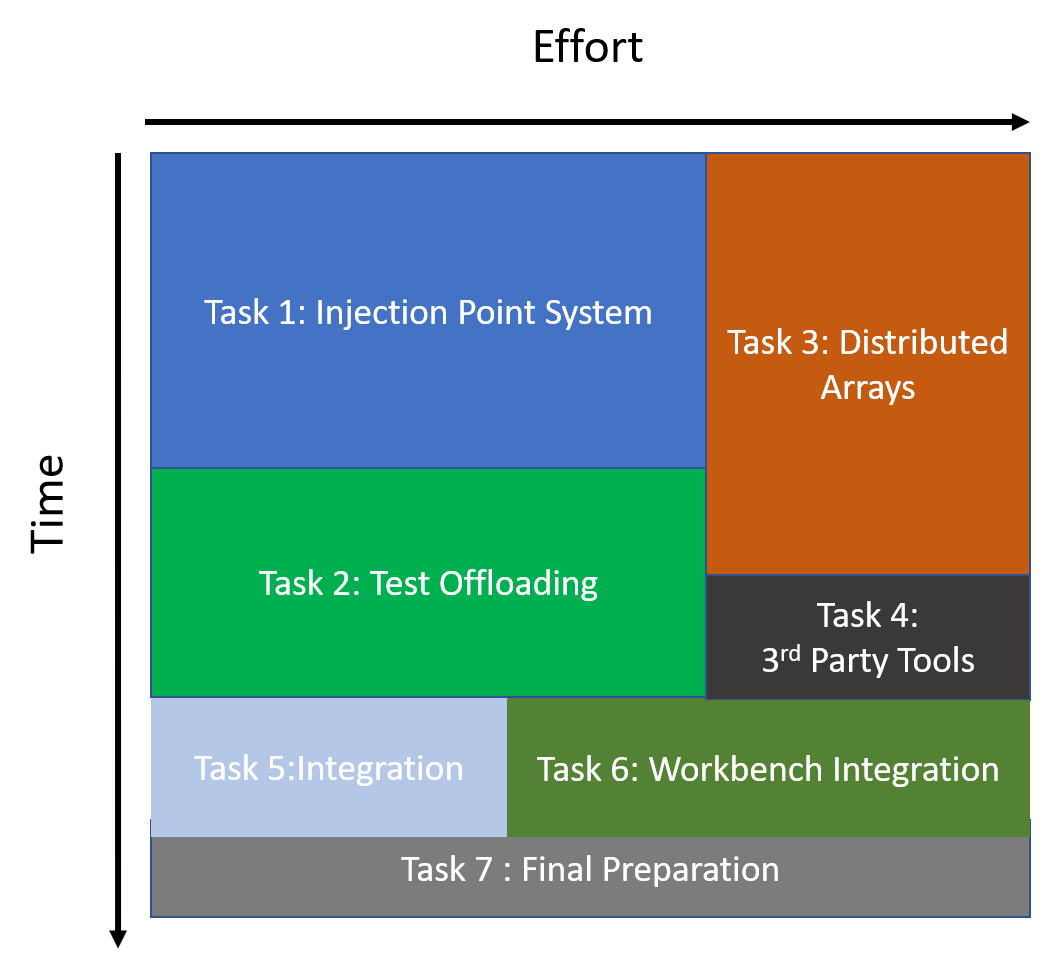
\includegraphics[width=1.0\linewidth]{./narrative/figures/tasks.pdf}
\end{center}
\caption{Overview of task dependencies and timeline.}
\label{fig:tasks}
\end{wrapfigure}

RNET would like to present the project ideas and research plan to the
DOE Program Manager and other interested scientists. The meeting will
be used to discuss features, and identify the specific NEAMS applications and computer
resources that will benefit from this project.  This meeting will be
scheduled soon after the Phase II contract is awarded. The meeting can
be hosted at RNET, a DOE site suggested by the Program Manager or via
a teleconference.

RNET will submit all reports as required by the contract (e.g., annual reports, 
a continuation report, summary reports, and a final report) to the DOE program 
manager and other interested DOE scientists.

The research and development topics described in Section~\ref{sec:workplan} 
will be addressed by the tasks described in the remainder of this section. Most 
tasks require active collaboration between RNET and its collaborators. 
Figure~\ref{fig:tasks} summarizes at a high level the dependencies among tasks  and
approximate anticipated task durations. The duration of the Phase II 
project is 104 weeks. Specific details are included in the description of each 
task.


\newcounter{taskCount}
\setcounter{taskCount}{0}

\refstepcounter{taskCount}\label{task:2.5}
\subsubsection{Task \ref{task:2.5}: Development of the Annotation based Inpjection Point System  }

In this task, the project team will develop the Annotation system for specifying injection points and describing injection variables. This will include the development of
the API for specifying the Annotations as shown in Figure~\ref{TODO}, and the development of the custom LLVM compiler extensions required to process these annotations. At the end of this task, users will be able to specify injection points and injection variables using either the new Annotation point system, or using the more portable, but less robust Phase I approach. 

To test the Annotation based injection point system, the project team will write injection points at several key locations in the MOOSE software stack, including inside the source code of several MOOSE modules, the core MOOSE framework, libMesh and PETSc. This will allow us to demonstrate the cross-library potential of the Annotation based system, while also acting as the first step toward integration of the tools a number of the NEAMS tools. 

\rnetprop{RNET will work on the implementation for this task and ORNL will provide inputs and guidance.}


\refstepcounter{taskCount}\label{task:3}
\subsubsection{Task \ref{task:3}: Develop methods for offloading tests to external processes. }

\refstepcounter{taskCount}\label{task:23}
\subsubsection{Task \ref{task:23}: Development of efficient statistical \VV tools with a focus of performance in large scale distributed settings.}


In this task, the project team will investigate the optimal approaches for conveying information about the data decompoosition to the individual tests. As outlined in Section~\ref{TODO}, this will involve the implementation of the BlockMap algorithm for data structures with regular decompositions and the implementation of a simple approach for generating the global partition for problems with irregular domain decompositions. Based on the performance of those implementations, the project team will investigate more optimal approaches to completing intra-processor communications with distributed data arrays, including creating a data directory or using the assumed partition algorithm 

In addition to this the project team will implement several statistical tools for asserting the state of the data in distributed arrays, as described in Section~\ref{TODO}. 

At the completion of this task, users will be able to efficiently compare and analyze distributed arrays using teh VnV framework. To test these implementations, the project team will set up tests for performing assertions on various PETSc vectors and matrices. The metric for success in this task will be to: (1) support arbitary data decompoistion descriptions; and (2) obtain a factor 5x speedup when performing assertions using our custom statistical assertions when compared to the naieve approach of gathering the data on a single root core for processing. 

\rnetprop{RNET will work on the implementation for this task and ORNL will provide inputs and guidance.}

\refstepcounter{taskCount}\label{task:22}
\subsubsection{Task \ref{task:22}: Development of Generic tools for Mesh refinement, Uncertainty quantification and Sensitivity Analysis.}
In this task, RNET will implement generic \VV tools for mesh refinement, uncertainty quantification and sensitivity analysis. In the case of mesh refinement, the approach taken will be to create a generic interface for interacting with the automatic mesh refinement functionality that already exists in finite element libraries like LibMesh and Fenics. The overall goal is to create a generic VnV test that can be attached to the main function of the executable such that it automates the process of running mesh refinement and mesh convergence studies. In the case of UQ and SA, the project team will develop an interface for specifying the tools available in DAKOTA as VnV tests. 

\rnetprop{RNET will be responsible for this task. ORNL will provide guidance on 
developing the framework for ORNL CADES.}


\refstepcounter{taskCount}\label{task:4}
\subsubsection{Task \ref{task:4}: Extension of the VnV report generation system}
In this task, the project team will complete the development of the VnV report generation system. he primary goal of this task will be
to provide support for generating VnV reports that conform to the specification outlined in the DoD VV report templates.  The task will also include  a full implementation 
of the VnV markdown extension to support a wide variety of data visualization components, the development of the interfaces required for displaying unit and regression testing
reports, and the software indirections required for assimilating multiple VnV reports into a single document that can be used in the \VV of an entire simulation package. 

\rnetprop{RNET will work on the implementation for this task}

\refstepcounter{taskCount}\label{task:1}
\subsubsection{Task \ref{task:1}: Integration into real applications, including the NEAMS Tools}
\rnetprop{
  In this task, the program team will integrate the VnV framework into a variety of real applications. Initially, this 
  testing will be completed in tools used heavily in the NEAMS toolkit; MOOSE, libMesh and PETSc, but other third party 
  applications will also be investigated. To ensure seamless integration with the MOOSE tools, the project team will reimplement
  the XML based configuration file using the MOOSE input file format. This will allow for the configuration of the VnV tests in 
  a MOOSE application directly from the input file.
  
  The goal of this task will be to generate informative, production quality VnV 
  reports for a number of examples available in the MOOSE testing suite. Doing so allows us
  to test every facet of the proposed framework, while also acting the first demonstration of the
  value provided by the framework. These results of these tests will be hosted on the RNET website 
  as they become available. 
 

}

\rnetprop{
RNET will be responsible for this task and ORNL will provide guidance on 
various technical implementations and details.
}
\refstepcounter{taskCount}\label{task:11}
\subsubsection{Task \ref{task:11}: Development of an interface for the NEAMS workbench}
\rnetprop{
  In this task, the project team will integrate the toolkit directly into the NEAMS workbench. This will be
  a two stage process. First, the project team will implement the required interface files for enabling 
  the context aware auto-complete features available in the NEAMS workbench for the MOOSE based configuration
  file specification developed in the previous section. MOOSE based input files are already largely supported in
  the workbench; however, there will likely be some issues with determining which tests are applicable at which 
  injection points. Second will be developing an interface for customizing and viewing the final VV report. As part of the Phase I
  effort, the project team demonstrated viewing the final \VV report in a QT WebView component. The workbench is also but on to
  off QT, hence we do not expect to many difficulties on that front. Instead the key objective will be to develop the mechanisms for
  displaying customizations made the the final report in real-time within the NEAMS workbench. 
}
\rnetprop{ RNET will be responsible for this task }


\subsection{Facilities/Equipment}
\subsubsection{RNET Facilities}
RNET has the necessary office equipment to manage an SBIR/STTR contract
including networks, workstations, and accounting software. In
addition, RNET has the tools (software and hardware) to evaluate and
develop the technologies proposed here.  

RNET currently has 9 development computers and a 10-node development cluster 
that can be used for development and testing in this effort. Each cluster node 
has two quad-core or hexa-core XEON CPUs, 24-32GB of DRAM, 500+GB of local 
disk. 
Two data networks are available, a COTS 1 Gbps Ethernet network and a 10 Gbps 
Ethernet network. The Linux development nodes and the RNET cluster have the 
necessary Linux/GNU toolchains and development environments including; GNU 
tool chain, Microsoft .Net Framework, and Java Standard Edition.

\subsubsection{ORNL Facilities}
%\rnetcomment{Jay to verify, can we state these resources can be used on this project?}
The Oak Ridge National Laboratory (ORNL) hosts three petascale computing 
facilities: the Oak Ridge Leadership Computing 
Facility (OLCF), managed for DOE; the National Institute for Computational 
Sciences (NICS) computing facility operated 
for the National Science Foundation (NSF); and the National Climate-Computing 
Research Center (NCRC), formed as 
collaboration between ORNL and the National Oceanographic and Atmospheric 
Administration (NOAA) to explore a variety of 
research topics in climate sciences. Each of these facilities has a 
professional, experienced operational and engineering 
staff comprising groups in high-performance computing (HPC) operations, 
technology integration, user services, scientific 
computing, and application performance tools.

%\rnetcomment{Ram: Based on Jay's comments.}
ORNL also has the Compute and Data Environment for Science (CADES) which is a 
fully integrated infrastructure offering compute and data services for 
researchers lab-wide. We will work with appropriate program managers to apply 
for allocation requests as appropriate.


 The ORNL computer facility staff 
provides continuous operation of the centers 
and immediate problem resolution. On evenings and weekends, operators provide 
first-line problem resolution for users with 
additional user support and system administrators on-call for more difficult 
problems. ORNL also has state-of-the-art 
visualization facilities that can be used on site or accessed remotely. 

\section{Consultants and Subcontractors}
Oak Ridge National Laboratory(ORNL) is the Research Institution for this proposal and will serve as a subcontractor for this SBIR. 

Jay Jay Billings, MS, is a Research Scientist at Oak Ridge National Laboratory where he leads the Scientific Software Development Team in the Computer Science and Mathematics Division.
%He holds the Bachelor’s Degree in Physics from Virginia Tech, class of 2005, and the Master of Science in Theoretical Astrophysics from the University of Tennessee, class of 2008.
Mr. Billings’ research focuses on the design and implementation of modeling and simulation tools for energy science, large parts of which has been related to the study of scientific workflows in an HPC context and computational physics. He was funded for eight years as a PI in the NEAMS program. At Oak Ridge National Laboratory, Mr. Billings is leading the new Scientific Software Initiative within the Division to take a new look at the way ORNL develops software for the Department of Energy. He is a founding member and current chair of the Science Working Group at the Eclipse Foundation, where he also leads the development of the Eclipse Integrated Computational Environment (ICE) and the Eclipse Advanced Visualization Project (EAVP). Mr. Billings was also appointed to the Eclipse Architecture Council in February 2016, and is a mentor for several additional Eclipse projects.

Mr. Billings has been funded by the Department of Energy Offices of Nuclear Energy (NE), Energy Efficiency and Renewable Energy (EERE), Advanced Scientific Computing Research (ASCR), and Advanced Manufacturing (AMO). In addition to his day job, Mr. Billings is a candidate for the PhD in Energy Science from the Bredesen Center for Interdisciplinary Research and Education at the University of Tennessee.% He spends his spare time with his wife, and singing.

Mr. Billings has extensive experience in creating a unified, integrated and dynamically reconfigurable environments in which analysts and developers can perform modeling and simulation tasks without having to deal with low-level command line utilities.

\section{Principal Investigator and other Key Personnel}
%{\em The Principal Investigator (PI) must be knowledgeable in all
%  technical aspects of the grant application and be capable of leading
%  the research effort and meet the requirements described in Part III,
%  C.  Describe the effort to be performed by the PI during the
%  project.}

\subsection{Ben O'Neill, PI}
Ben O'Neill is a Research Scientist at RNET and will be the PI on this project. Ben is a full time employee at
RNET and has sufficient time to dedicate to this project. Ben is a permanent resident in the USA (citizen of New Zealand). The proposed work does not include any Export Control restriction, as such, this work visa should be sufficient. In addition to the current project, Ben is the lead developer in RNET's
Cloudbench project which aims to develop a web-enabled interface for remote execution and visualization for nuclear physics tools. Ben was also heavily involved in the development of the SolverSelector framework for facilitating automatic linear solver selection in high performance applications through machine learning. His background is in Applied mathematics with a focus on high performance computing and parallel-time integration. His thesis work involved the optimization and implementation of a parallel time integration codes for nonlinear PDEs including implementing a fully adaptive and parallel space-time solver using the Fenics finite element package.

\subsection{Gerald Sabin}
Dr. Gerald Sabin, Project Manager at RNET, will be the senior advisor for this project.
Dr.  Sabin is a full time employee of RNET, and has sufficient time to dedicate to project tasks as indicated in the
cost proposal. Since he is a US Citizen, he can undertake relevant
integration work in Export-Controlled areas of the project, if
necessary. Currently, he is working on several Scientific Computing
(HPC) SBIR/STTR projects at RNET. He is the PI for this Phase II SBIR
Cloudbench project (DE-SC0015748) and the ongoing Phase II DOE SBIR for the Automated Solver Selection for Nuclear
Engineering Simulations. He has also worked on distributed memory,
GPU, multi-core and SIMD optimizations to the Air Force's Kestrel code
(DOD Contract\#:FA9550-12-C-0028) and has also been involved in
developing fine-grained power profiling hardware and software tools
for HPC application profiling (DOE Contract\#:DE-SC0004510). He has
also been the PI on several other related projects including a NASA
Phase I project developing SIMD optimizations for Monte Carlo codes
(NNX14CA44P), developing parallelization optimizations for PETSc (DOE
Contract\#: DE-SC0002434), developing data virtualization support and
bitmap indexing for massive Climate Modeling data sets (DOE Contract
\#:DE-SC0009520), and developing the SmartNIC software stack for
application-aware network offloading (DOE Contract\#:
DE-FG02-08ER86360).


\section{Related Work}
\label{related}

RNET and ORNL have past and current experience in several SBIR/STTR projects on modeling and simulation, high performance computing, 
and large data formats. Some of these projects are briefly described below. 

\subsection{RNET's Related Work}

\subsubsection{Automated Solver Selection for NEAMS Tools}

RNET in collaboration with University of Oregon (Dr. Boyana Norris) is developing an add-in feature for the NEAMS 
toolkit being developed by the Department of Energy. This work is being done as part of DOE Phase II STTR project 
(Contract Number DE-SC0013869). This add-in feature being developed by RNET leverages machine learning techniques 
to automatically select the optimal solver based on run-time dependent features of the problem and the underlying 
compute architecture with minimal runtime overhead in solver selection during the course of NEAMS simulations. 


\subsubsection{Cloud-based Scientific Workbench for Nuclear Reactor Simulation Life Cycle Management}
The predictive modeling approaches and softwares being continually developed and updated by the DOE nuclear engineering scientists (under programs such as NEAMS, CASL, RISMC etc.) need to be efficiently transferred to the nuclear science and engineering community. An advanced workflow management workbench is required to allow efficient usage from small and large business and research groups. The workbench must manage inputs decks, simulation execution (on a local machine, a High Performance Compute cluster, or a Cloud cluster), intermediate results, final results and visualizations, and provenance of the tools and settings. CloudBench is a hosted simulation environment for large scale numeric simulations. CloudBench will augment existing simulation, Integrated Development Environment, and workbench tools being developed by the DOE and industry. It offers a complete set of simulation management features not available in open tools: sharing of configurations, simulation output, and provenance on a per simulation or per project basis; multi-simulation provenance history to allow simulations to be reconstructed, verified, or extended; and remote access to simulation tools installed on Cloud and HPC resources. The portal enables easy adoption of government codes. 

%% \subsubsection{Catalytic Converter Modeling on High-End Workstations}

%% RNET Technologies, Inc. in collaboration with Prof. Sandip Mazumder developed performance optimizations for accurate 
%% CFD simulation of full-scale monolithic catalytic converters as an alternative to extrapolating single channel simulation 
%% to the entire monolith \cite{Choudary1}. This project has been funded by Department of Energy under the STTR program 
%% (Contract Number DE-SC 0007580). A numerical method (and code), recently developed at OSU, that successfully demonstrated 
%% simulation of laboratory-scale catalytic converters with realistic surface chemistry has been revamped and optimized for 
%% industrial-scale simulations. The enhancements made to the existing method included rewriting certain functionalities to 
%% multicore processors and GPGPUs. Using these performance optimizations, a speedup of ~4.5X has been achieved for 3D test 
%% problems with 300K cells, 20+ reactions, and various mesh topologies. These optimizations will facilitate Catalytic 
%% Converter Simulation on high-end workstations and small clusters by fully utilizing the compute resources (Multicores, 
%% GPUs, vector processing units, etc.) in emerging architectures. 

\subsubsection{Scaling the PETSc Numerical Library to Petascale Architectures}

RNET has developed an extended version of the numerical library PETSc \cite{Lowell1} in
collaboration with Ohio State University and Argonne National Lab. PETSc is an MPI-based numerical library of
linear and nonlinear solvers that is widely used in a variety of scientific domains. With the
emergence of multicore processors and heterogeneous accelerators as the building blocks of
parallel systems, it is essential to restructure the PETSc code to effectively exploit multi-level
parallelism. Changes to the underlying PETSc data structures are required to leverage the multicore
nodes and GPGPUs being added to the ``cluster architectures''.

This project was funded by Department of Energy under the STTR program from August 2010 (Contract Number DE-SC0002434) 
to May 2013. Dr. P. Sadayappan (OSU) and Dr. Boyana Norris (ANL) have played a key role in this effort by serving as 
technical advisors. As part of the project, the team has investigated ways for the PETSc library to fully utilize the 
computing power of future Petascale computers. Novel sparse matrix types,  vector types, and preconditioning techniques 
that are conducive for GPU processing and SIMD parallelization have been integrated into the PETSc library. The matrix 
vector operations have been optimized for specific architectures and GPUs by utilizing the autotuning tools.


\subsubsection{Optimization of Kestrel for Emerging Architectures}
RNET and OSU are performing this work as part of an active DOD Phase
II STTR (FA9550-12-C-0028, Highly-Scalable Computational-Based
Engineering). Based on the identification of the main performance
bottlenecks in the Kestrel CFD code (based on the AVUS CFD solver), we
are developing enhancements to improve the performance of the kCFD
solver, as well as interface other scalable Krylov subspace sparse
solver libraries to Kestrel. The proposed work will address the
effective exploitation of parallelism at multiple levels: SIMD/SIMT
level, multi-core level, and multi-node level.

As part of this project CUDA kernels are also being explored for the
bottlenecks in the CFD and CSD solvers. For instance, a GPU-based CFD
solver with an identical interface to the current Block-Seidel solver
is being explored.



\subsection{ORNL's Related Work}
%\subsubsection{ICE}
\label{sec:nice}

Dr. Watson is the main developer for the Eclipse Parallel Tools Platform (PTP). The aim of the PTP project is to produce an open-source industry-strength platform that provides a highly integrated environment specifically designed for parallel application development. The platform provides a standard, portable parallel IDE that supports a wide range of parallel architectures and runtime systems; a scalable parallel debugger; support for the integration of a wide range of parallel tools; and an environment that simplifies the end-user interaction with parallel systems. 

In addition, Dr. Watson has played a significant role in the development of GAURD, a parallel relative debugger for high performance systems. Unlike other conventional parallel debuggers a relative debugger provides the
ability to dynamically compare data between two executing programs regardless of their location and configuration. In GAURD, data
comparisons can be performed either using an imperative scheme or a declarative scheme. Imperative comparisons can be performed
explicitly by the user when two programs under the control of the debugger are stopped at breakpoints. 

A solid foundation has been laid to achieve the objectives of the proposed project. The final 
 piece of the puzzle is the optimization and hardening of these core approaches for efficient execution in real applications. 
 Once this is accomplished, it will be possible to seamlessly integrate functionality for end-user \VV into any general purpose 
 numerical simulation software. The collaboration between ORNL and 
RNET is a perfect fit to facilitate this final step. RNET brings to the table the required computer science expertise to 
satisfy the needs of this project, as is evident from a description of their related work, and ORNL brings a wealth of experience developing novel
HPC software solutions, developing robust debugging tools for use in HPC environments and working with a range of real application codes. 

